\chapter{Design and Implementation}
\label{chap:DesignImplementation}

\section{Architecture}

\subsection{Static view}

\newpage

\begin{figure}[h]
    \centering
    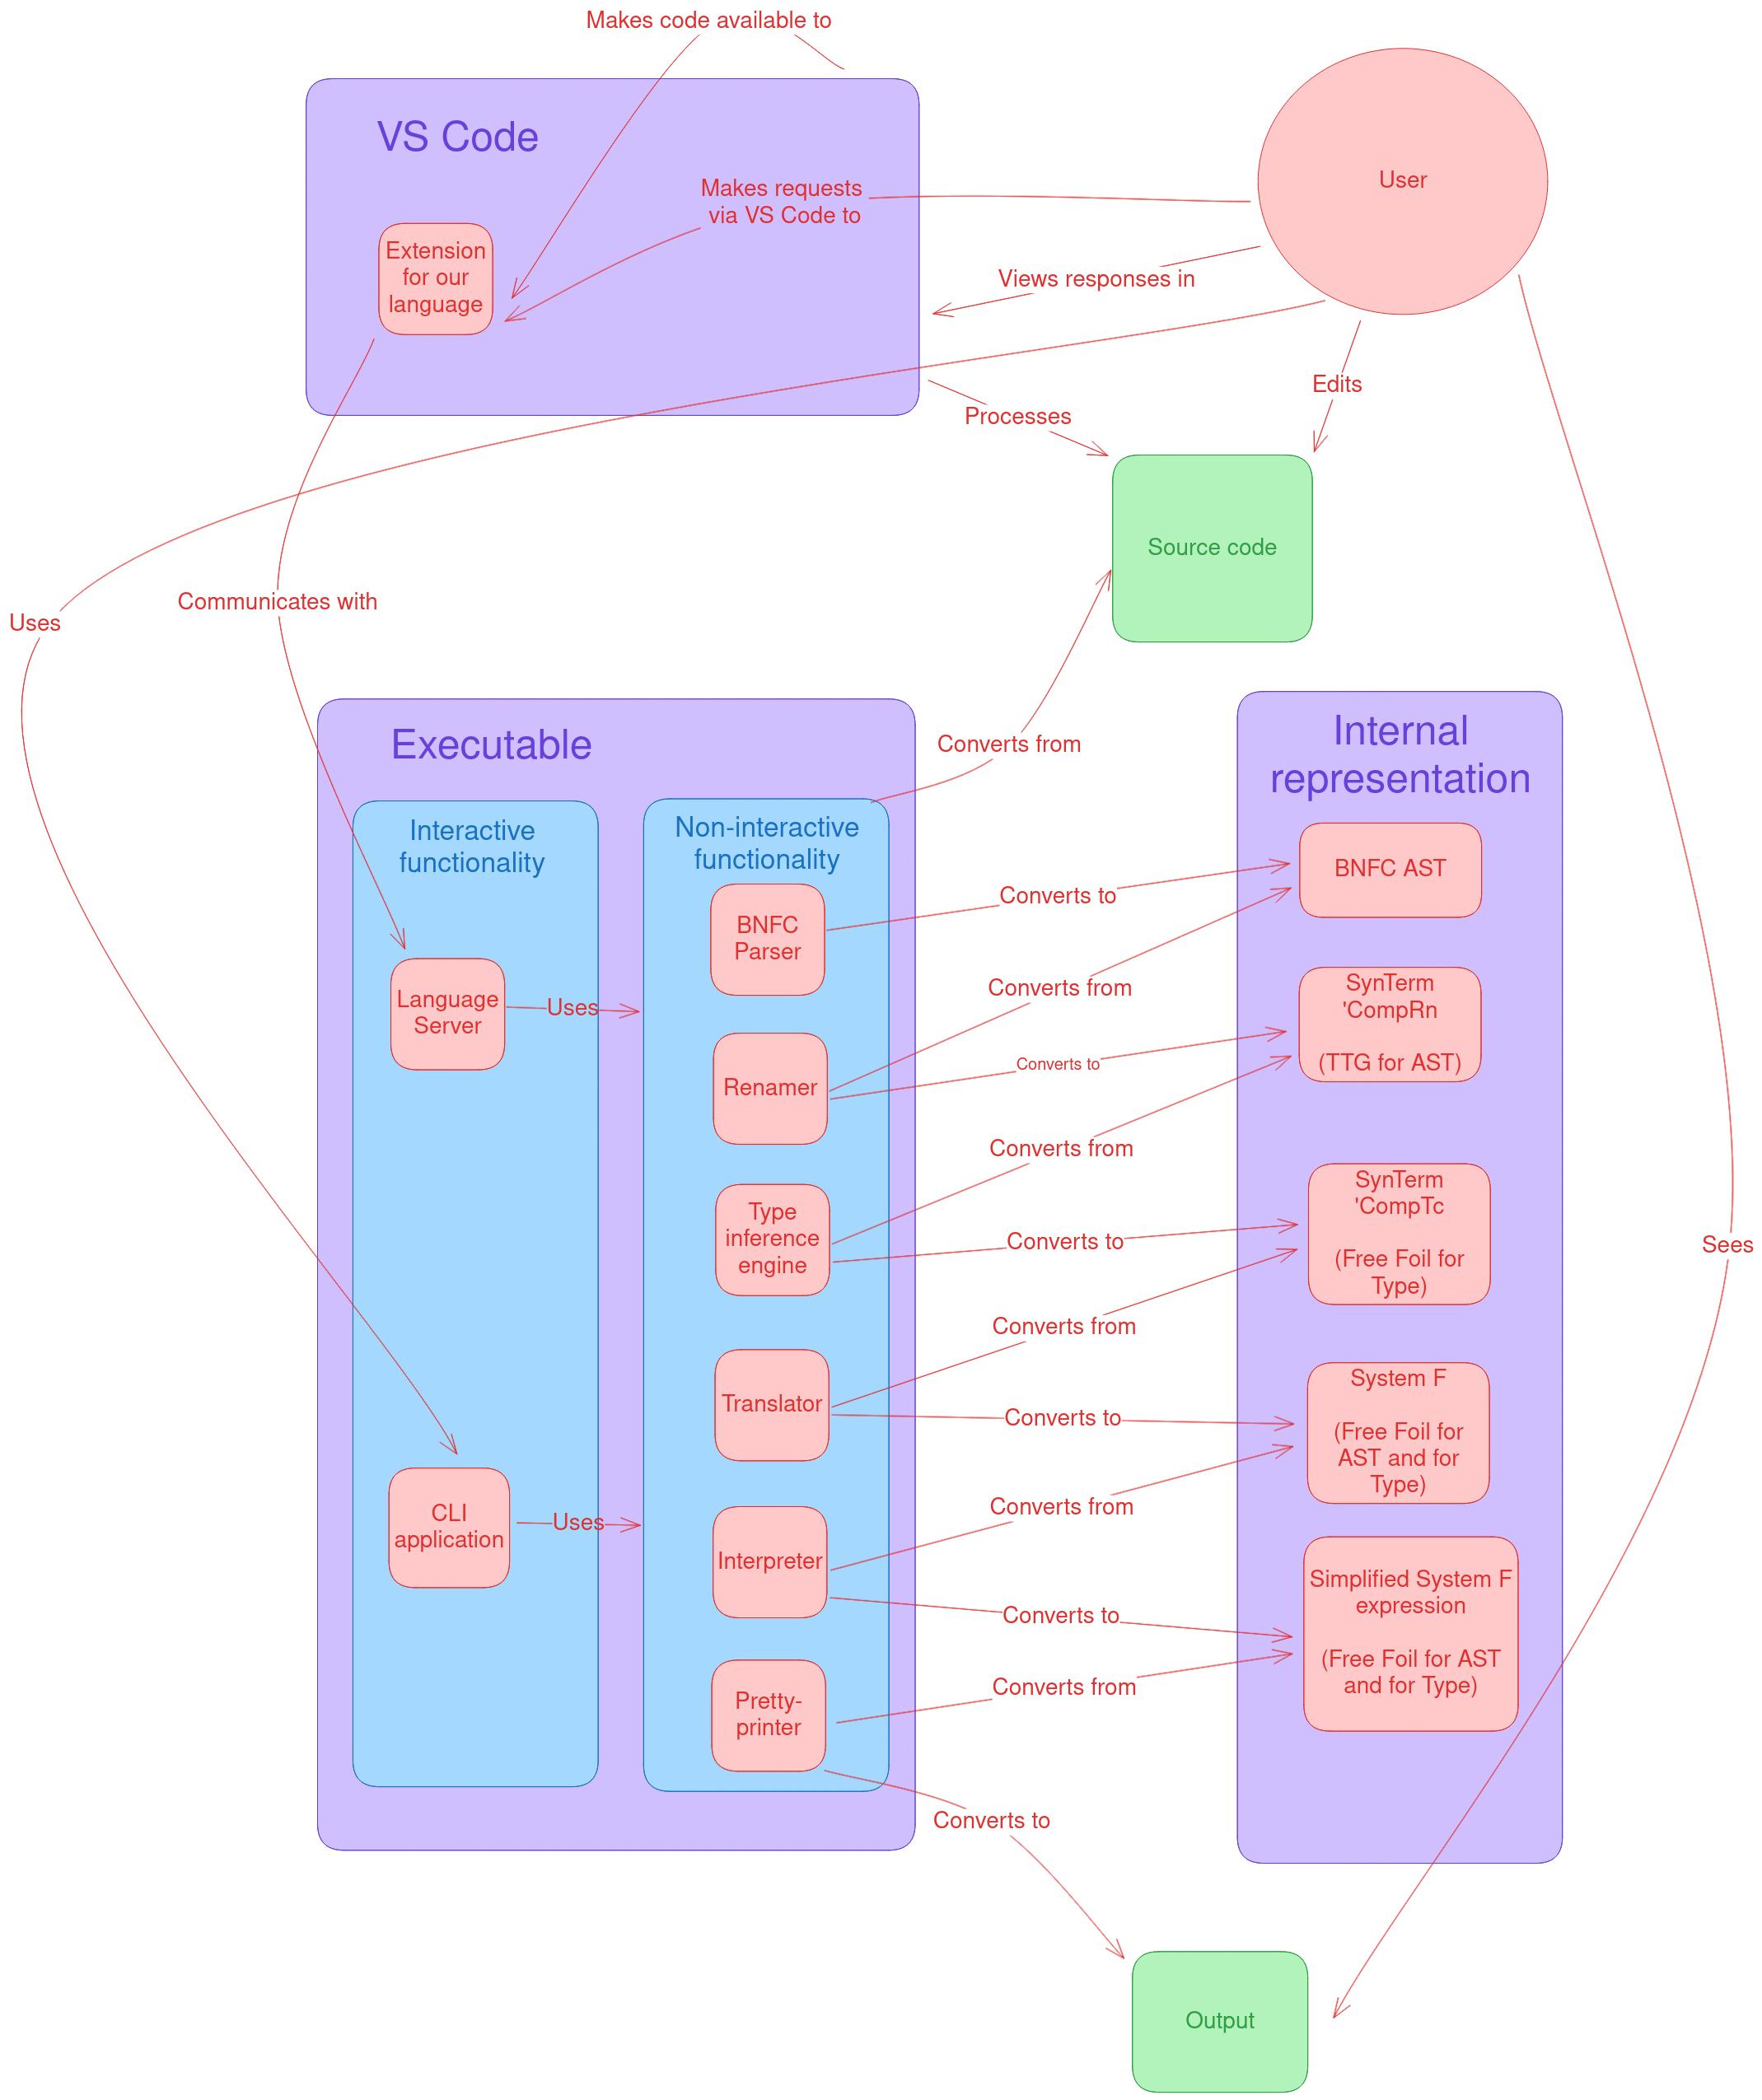
\includegraphics[scale=0.25]{Architecture.png}
    \caption{Static view}
    \label{Architecture}
\end{figure}

\newpage

\subsection{Use Case: Interpreter is called.}

\subsubsection{Parsing}

A BNFC-generated parser reads the source code written in our language and produces a raw BNFC AST with positions of tokens.

\subsubsection{Renaming}

The raw BNFC AST is then converted to the Trees That Grow representation \texttt{SynTerm 'CompRn}.
During conversion, positions are copied to annotations and each variable in the program gets a unique identifier under condition.
Same variables appearing in multiple places in the program get the same identifiers.

\subsubsection{Typing}

The typing algorithm runs.
It uses the Free Foil representation of Core Types.
The typing algorithm annotates the tree with fully instantiated (not having metavariables) types producing \texttt{SynTerm 'CompTc} or throwing an error.

\subsubsection{Translation to System F}

The \texttt{SynTerm 'CompTc} is converted to the System F syntax using the Free Foil representation.

\subsubsection{Interpretation}

The interpreter evaluates the System F code.

\subsubsection{Output}

The program pretty-prints the resulting expression.

\subsection{Use case: user queries a type of a variable.}

\subsubsection{Start language server}

VS Code extension starts the language server if not started.
VS Code extension makes the language server read the code in the current file.

\subsubsection{Query}

VS Code extension passes a position to the language server and asks for the type of the variable at that position.

\subsection{Process}

The language server updates the AST if necessary, performs type checking, finds the node at the given position, and returns its type to the extension.

\section{AST}

We used the Trees That Grow approach \cite{trees-that-grow-2016} for the AST representation.

In GHC, some fields are just types constructed using the index parameter. In contrary, we used type family applications to the index parameter in all fields of the AST to make the AST more flexible. Additionally, we named the type families and constructors consistently to improve code navigation.

\begin{minted}{haskell}
-- GHC

-- Language/Haskell/Syntax/Expr.hs

data HsExpr p
  = HsVar     (XVar p)
              (LIdP p)
    ...

-- Language/Haskell/Syntax/Extension.hs

type LIdP p = XRec p (IdP p)

-- Ours

-- Language/STLC/Typing/Jones2007/BasicTypes.hs

data SynTerm x
    = -- | variables
      SynTerm'Var (XSynTerm'Var' x) (XSynTerm'Var x)
    ...

-- The Name already contains an SrcSpan, so it doesn't need an annotation
type instance XSynTerm'Var x = Name
\end{minted}

Like in GHC, we had separate data types that represented syntactic types and types used during typing.

\begin{minted}{haskell}
-- Ours

-- Language/STLC/Typing/Jones2007/BasicTypes.hs

data SynType x
  = -- | Type variable
    SynType'Var (XSynType'Var' x) (XSynType'Var x)
    ...

data Type
  = -- | Vanilla type variable.
    Type'Var Var
  ...
\end{minted}


TODO use the Free Foil representation for Type
TODO Free foil - try to marry with indices assigned by the Tc monad
TODO write about the type system.

% perform typing on a slightly desugared AST.
% We used the Free Foil representation of the Core types.

% TODO schema

% Free foil - try to marry with indices assigned by the monad